\begin{frame}
    \frametitle{Sistemas de equações lineares}
    Um sistema de equações lineares consiste em um conjunto de $m$ equações lineares com $n$ variáveis de $x_i$:

    \begin{align*}
        a_{11} x_1 + a_{12} x_2 + a_{13} x_3 + \cdots  + a_{1n} x_n & =  b_1 \\
        a_{21} x_1 + a_{22} x_2 + a_{23} x_3 + \cdots + a_{2n} x_n & =  b_2 \\
        a_{31} x_1 + a_{32} x_2 + a_{33} x_3 + \cdots + a_{3n} x_n & = b_3 \\
                                                                   & ~\vdots~ \\
        a_{m1} x_1 + a_{m2} x_2 + a_{m3} x_3 + \cdots  + a_{mn} x_n & =  b_m
    \end{align*}
\end{frame}

\begin{frame}
    \frametitle{Sistema de equações lineares - forma matricial}
    O sistema anterior pode ser representado na forma matricial por:

    \[
        \begin{bmatrix}
            a_{11} & a_{12} & a_{13} & \cdots & a_{1n}  \\
            a_{21} & a_{22} & a_{23} & \cdots & a_{2n}  \\
            a_{31} & a_{32} & a_{33} & \cdots & a_{3n}  \\
                   &        &        & \vdots &         \\
            a_{m1} & a_{m2} & a_{m3} & \cdots & a_{mn}
        \end{bmatrix}
        \begin{bmatrix}
            x_1 \\ x_2 \\ x_3 \\ \vdots \\ x_n
        \end{bmatrix}=
        \begin{bmatrix}
            b_1 \\ b_2 \\ b_3 \\ \vdots \\ b_m
        \end{bmatrix}
    \]

    ou simplesmente $Ax=b$, onde $A$ é chamada de matriz de coeficientes, $x$ é o vetor solução e $b$ é o vetor dos termos independentes. Resolver um sistema consiste em encontrar um vetor $x$ que satisfaça simultaneamente às equações.

    \pause

    Se $A$ for uma matriz quadrada ($m = n$) não singular ($det(A) \neq 0$), então:

    \[
        Ax=b ~\rightarrow~ A^{-1}Ax=A^{-1}b ~\rightarrow~ x=A^{-1}b
    \]
\end{frame}

\begin{frame}
    \frametitle{Sistema triangular superior}

    Seja um sistema triangular superior 3x3
    \[
        \begin{bmatrix}
            a_{11} & a_{12} & a_{13} \\
            0      & a_{22} & a_{23} \\
            0      & 0      & a_{33}
        \end{bmatrix}
        \begin{bmatrix}
            x_1 \\ x_2 \\ x_3
        \end{bmatrix}
        =
        \begin{bmatrix}
            b_1 \\ b_2 \\ b_3
        \end{bmatrix}
    \]

    O vetor solução \( x\) pode ser obtido através de substituições retroativas:
    \begin{align*}
        x_3 &= \frac{b_3}{a_{33}} \\
        x_2 & = \frac{b_2 - a_{23}x_3}{a_{22}} \\
        x_1 &= \frac{b_1 - a_{12}x_2 - a_{13}x_3}{a_{11}}
    \end{align*}
\end{frame}

\begin{frame}
    Ou seja,

    \[
        x_i = \frac{b_i - \sum_{j=i+1}^{3} {a_{ij} x_j}}{a_{ii}}
    \]
    onde \(i = 3, 2, 1\). Para um sistema \(n\) x \(n\), temos
    \[
        x_i = \frac{b_i - \sum_{j=i+1}^{n} {a_{ij} x_j}}{a_{ii}}
    \]
    onde \(i = n, n-1, n-2, \ldots , 1\)

    \begin{block}{Eliminação de Gauss}
        O método de eliminação de Gauss consiste em transformar um sistema de equações lineares em um sistema triangular superior equivalente e obter o vetor solução através de substituições retroativas
    \end{block}
\end{frame}

\begin{frame}
    Um sistema linear pode ser transformado em outro equivalente através das operações
    \begin{itemize}
        \item Trocar a ordem de duas equações
        \item Multiplicar uma equação por uma constante não nula
        \item Somar duas equações
    \end{itemize}

    \begin{block}
        {Exemplo}
        Resolva o seguinte sistema usando eliminação de Gauss

        \[
            \begin{bmatrix}
                10 & 3 & -2 \\ 2 & 8 & -1 \\ 1 & 1 & 5
            \end{bmatrix}
            \begin{bmatrix}
                x_1 \\ x_2 \\ x_3
            \end{bmatrix}
            =
            \begin{bmatrix}
                57 \\ 20 \\ -4
            \end{bmatrix}
        \]

    \end{block}
\end{frame}

\begin{frame}
    \frametitle{Primeira etapa}
    Como as operações envolvem as equações, tanto \(A\) quanto \(b\) são modificadas. Assim, é interessante construir uma matriz ''aumentada'' \([A,b]\):

    \[
        [A,b] =
        \left[
            \begin{array}{ccc|c}
                10 & 3 & -2 & 57 \\ 2 & 8 & -1 & 20 \\ 1 & 1 & 5 & -4
            \end{array}
        \right]
    \]

    de maneira que as operações ocorrendo em \(A\) também ocorram em \(b\).

    \begin{block}
        {}
        Em uma matriz triangular superior, todos os elementos abaixo da diagonal são nulos. Assim, devemos zerar todos os elementos abaixo da diagonal
    \end{block}

\end{frame}

\begin{frame}
    \frametitle{Segunda etapa}

    \begin{enumerate}
        \item ''Somamos'' a segunda equação (\(L_2\)) com a primeira (\(L_1\)) multiplicada por uma constante, de forma que o elemento \(a_{21} = 0\)
            \[
                L_2 \leftarrow L_2 - \frac{a_{21}}{a_{11}} L_1
            \]
        \item ''Somamos'' a terceira equação (\(L_3\)) com a primeira (\(L_1\)) multiplicada por uma constante, de forma que o elemento \(a_{31} = 0\)
            \[
                L_3 \leftarrow L_3 - \frac{a_{31}}{a_{11}} L_1
            \]
    \end{enumerate}
    \[
        \left[
            \begin{array}{ccc|c}
                10 & 3 & -2 & 57 \\ 2 & 8 & -1 & 20 \\ 1 & 1 & 5 & -4
            \end{array}
        \right]
        \rightarrow
        \left[
            \begin{array}{ccc|c}
                10 & 3 & -2 & 57 \\ 0 & 37/5 & -3/5 & 43/5 \\ 0 & 7/10 & 26/5 & -97/10
            \end{array}
        \right]
    \]
\end{frame}

\begin{frame}
    \frametitle{Terceira etapa}
    \begin{enumerate}
        \item ''Somamos'' a terceira equação (\(L_3\)) com a segunda (\(L_2\)) multiplicada por uma constante, de forma que o elemento \(a_{32} = 0\)
            \[
                L_3 \leftarrow L_3 - \frac{a_{32}}{a_{22}} L_2
            \]
    \end{enumerate}
    \[
        \left[
            \begin{array}{ccc|c}
                10 & 3 & -2 & 57 \\ 0 & 37/5 & -3/5 & 43/5 \\ 0 & 7/10 & 26/5 & -97/10
            \end{array}
        \right]
        \rightarrow
        \left[
            \begin{array}{ccc|c}
                10 & 3 & -2 & 57 \\ 0 & 37/5 & -3/5 & 43/5 \\ 0 & 0 & 389/74 & -389/37
            \end{array}
        \right]
    \]
\end{frame}

\begin{frame}
    \frametitle{Quarta etapa}
    Resolvemos o sistema triangular superior usando a expressão
    \[
        x_i = \frac{b_i - \sum_{j=i+1}^{n} {a_{ij} x_j}}{a_{ii}}
    \]
    onde \(i = n, n-1, n-2, \ldots , 1\)

    \begin{align*}
        x_3 &= \frac{-389/37}{389/74}=-2 \\
        x_2 & =\frac{43/5 - (-3/5)*(-2)}{37/5}=1 \\
        x_1 &= \frac{57-3*1-(-2)*(-2)}{10} = 5
    \end{align*}

\end{frame}


\begin{frame}{Sistema de equações lineares - planilha eletrônica}
    \begin{itemize}
        \item Seja o sistema na forma matricial \(Ax=b\):
            \[
                \begin{bmatrix}
                    a_{11} & a_{12} & a_{13} & \cdots & a_{1n}  \\
                    a_{21} & a_{22} & a_{23} & \cdots & a_{2n}  \\
                    a_{31} & a_{32} & a_{33} & \cdots & a_{3n}  \\
                           &        &        & \vdots &         \\
                    a_{m1} & a_{m2} & a_{m3} & \cdots & a_{mn}
                \end{bmatrix}
                \begin{bmatrix}
                    x_1 \\ x_2 \\ x_3 \\ \vdots \\ x_n
                \end{bmatrix}=
                \begin{bmatrix}
                    b_1 \\ b_2 \\ b_3 \\ \vdots \\ b_m
                \end{bmatrix}
            \]
        \item Como vimos, podemos resolvê-lo encontrando a matriz inversa de \(A\)
            \[
                Ax=b \implies x=A^{-1}b
            \]
        \item Para matrizes pequenas, podemos usar as funções \texttt{MATRIZ.MULT} e \texttt{MATRIZ.INVERSO}
    \end{itemize}
\end{frame}

\begin{frame}[c]{Planilha eletrônica}

    \begin{itemize}
        \item Temos que \(Ax=b ~\rightarrow~ A^{-1}Ax=A^{-1}b ~\rightarrow~ x=A^{-1}b\)
        \item A função \texttt{MATRIZ.MULT(matriz1; matriz2)} multiplica duas matrizes
        \item A função \texttt{MATRIZ.INVERSO(matriz\_quadrada)} calcula a inversa de uma matriz quadrada
        \item Se colocarmos a matriz \(A\) nas células \texttt{A1:G7} e a matriz \(b\) em \texttt{H1:H7}, a matriz \(x\) pode ser calculada por
            \begin{center}
                \texttt{=MATRIZ.MULT(MATRIZ.INVERSO(A1:G7);H1:H7)}
            \end{center}
    \end{itemize}

\end{frame}

\begin{frame}[c]{Mas nem tudo são flores...}
    Essas funções têm particularidades dependendo da planilha
    \begin{itemize}
        \item \textbf{LibreOffice}: para finalizar a entrada do comando você deve digitar \texttt{Ctrl-Shift-Enter} ao invés de apenas \texttt{Enter}
        \item \textbf{Excel}: antes de entrar o comando você deve selecionar o número de células que serão ocupadas e para finalizar a entrada do comando você deve digitar \texttt{Ctrl-Shift-Enter} ao invés de apenas \texttt{Enter}
        \item \textbf{Google Planilhas}: para finalizar a entrada do comando você deve digitar \texttt{Ctrl-Shift-Enter} seguido de \texttt{Enter} ao invés de apenas \texttt{Enter}
    \end{itemize}

\end{frame}

\begin{frame}{Exercícios extras}
    Encontre as soluções dos sistemas lineares abaixo usando uma planilha eletrônica:

    \begin{columns}
        \begin{column}{0.45\textwidth}
            \begin{enumerate}
                \item \systeme*{-4x+2y=5,-x-9y+5z=6,x-3y+4z=9}
                \item \systeme*{6x-y-8z=-5,-6x+4y-2z=7,4x+9y-8z=-7}
                \item \systeme*{x-5y+9z=5,y-z=-8,8x-3y+6z=-3}
            \end{enumerate}
        \end{column}

        \begin{column}{0.45\textwidth}
            \begin{enumerate}\addtocounter{enumi}{3}
                \item \systeme*{-t-5u+8v+6w=-3,3t+u+4v-w=6,-6t-u+8v-5w=6,-7t+3u-3v=3}
                \item \systeme*{2t+9u+8v+4w=4,-9t-8u-9v+9w=-5,-7t-7u+2v+4w=-5,3t+6u=4}
            \end{enumerate}
        \end{column}
    \end{columns}

\end{frame}

\begin{frame}
    \frametitle{Sistemas não lineares}

    O sistema a seguir é formado por um conjunto de duas equações simultâneas não lineares com duas incógnitas
    \[
        \begin{cases}
            x_1^2 + x_1x_2 &= 10 \\
            x_2 + 3x_1x_2^2 &= 57
        \end{cases}
    \]

    Podemos expressar esse sistema na forma

    \[
        \begin{cases}
            x_1^2 + x_1x_2 -10 &= 0 \\
            x_2 + 3x_1x_2^2 -57 &= 0
        \end{cases}
    \]

    ou seja: a solução do sistema são os os valores de $x_1$ e $x_2$ que tornam as equações iguais a zero
\end{frame}

\begin{frame}[c]
    De forma geral, qualquer sistema não linear pode ser expresso na forma
    \[
        \begin{cases}
            f_1(x_1, x_2, \ldots, x_n) =& 0 \\
            f_2(x_1, x_2, \ldots, x_n) =& 0 \\
            \vdots & \\
            f_n(x_1, x_2, \ldots, x_n) =& 0 \\
        \end{cases}
    \]

    e para encontrar a solução basta encontrar os zeros das funções. O problema reside no fato de $f_1$, $f_2$, $\ldots$, $f_n$ serem funções de mais de uma variável
\end{frame}

\begin{frame}
    \frametitle{Método de Newton-Raphson}
    Devemos definir um vetor solução inicial $x^0$ e encontrar o vetor solução $x^{k+1}$ através da fórmula
    \[
        \color{blue}
        x^{k+1}=x^k-J^{-1} f
    \]
    onde

    \[
        \color{red}
        J=
        \begin{bmatrix}
            \left. \dfrac{\partial f_1}{\partial x_1}\right\rvert_{x_1^k,x_2^k,\ldots,x^k_N} &
            \left. \dfrac{\partial f_1}{\partial x_2}\right\rvert_{x_1^k,x_2^k,\ldots,x^k_N} & \ldots &
            \left. \dfrac{\partial f_1}{\partial x_N}\right\rvert_{x_1^k,x_2^k,\ldots,x^k_N} \\
            \left. \dfrac{\partial f_2}{\partial x_1}\right\rvert_{x_1^k,x_2^k,\ldots,x^k_N} &
            \left. \dfrac{\partial f_2}{\partial x_2}\right\rvert_{x_1^k,x_2^k,\ldots,x^k_N} & \ldots &
            \left. \dfrac{\partial f_2}{\partial x_N}\right\rvert_{x_1^k,x_2^k,\ldots,x^k_N} \\
            \vdots & \vdots & \ddots & \vdots \\
            \left. \dfrac{\partial f_N}{\partial x_1}\right\rvert_{x_1^k,x_2^k,\ldots,x^k_N} &
            \left. \dfrac{\partial f_N}{\partial x_2}\right\rvert_{x_1^k,x_2^k,\ldots,x^k_N} & \ldots &
            \left. \dfrac{\partial f_N}{\partial x_N}\right\rvert_{x_1^k,x_2^k,\ldots,x^k_N}
        \end{bmatrix}
        \color{black}
        \text{ e }
        \color{magenta}
        f=
        \begin{bmatrix}
            f_1(x_1^k,x_2^k,\ldots,x^k_N) \\
            f_2(x_1^k,x_2^k,\ldots,x^k_N) \\ \vdots \\
            f_N(x_1^k,x_2^k,\ldots,x^k_N)
        \end{bmatrix}
    \]

\end{frame}

\begin{frame}
    \frametitle{Exemplo}
    O sistema
    \[
        \begin{cases}
            x_1^2 + x_1x_2 &= 10 \\
            x_2 + 3x_1x_2^2 &= 57
        \end{cases}
    \]
    tem

    \begin{columns}[T]
        \begin{column}{0.45\textwidth}
            \[
                J=
                \begin{bmatrix}
                    2x_1 + x_2 & x_1 \\
                    3x_2^2 & 1 + 6x_1x_2
                \end{bmatrix}
            \]
        \end{column}

        \begin{column}{0.45\textwidth}

            \[
                f=
                \begin{bmatrix}
                    x_1^2 + x_1x_2 - 10 \\
                    x_2 + 3x_1x_2^2 - 57
                \end{bmatrix}
            \]
        \end{column}
    \end{columns}

    Usando
    \[
        x^0=
        \begin{bmatrix}
            1,5 \\ 3,5
        \end{bmatrix}
    \]
    temos

    \begin{columns}
        \begin{column}{0.45\textwidth}
            \[
                J=
                \begin{bmatrix}
                    6,5 & 1,5 \\
                    36,75 & 32,5
                \end{bmatrix}
            \]
        \end{column}

        \begin{column}{0.45\textwidth}
            \[
                f=
                \begin{bmatrix}
                    -2,5 \\
                    1,625
                \end{bmatrix}
            \]
        \end{column}
    \end{columns}
\end{frame}

\begin{frame}[c]
    Usando \texttt{MATRIZ.INVERSO}, temos que
    \[
        J^{-1}=
        \begin{bmatrix}
            0,2082 &	-0,0096 \\
            -0,2354	& 0,0416  \\
        \end{bmatrix}
    \]

    e
    \[
        \begin{bmatrix}
            x_1^1 \\ x_2^1
        \end{bmatrix}
        =
        \begin{bmatrix}
            1,5 \\ 3,5
        \end{bmatrix}
        -
        \begin{bmatrix}
            0,2082 &	-0,0096 \\
            -0,2354	& 0,0416  \\
        \end{bmatrix}
        \begin{bmatrix}
            -2,5 \\
            1,625
        \end{bmatrix}
        =
        \begin{bmatrix}
            2,0360 \\
            2,8439
        \end{bmatrix}
    \]
\end{frame}

\begin{frame}{Exemplo}
    Resolva o seguinte sistema não linear
    \[
        \begin{cases}
            x_1^2+x_2^2+x_3^2=1 \\
            2x_1^2+x_2^2-4x_3=0 \\
            3x_1^2-4x_2+x_3=0
        \end{cases}
    \]
    com
    \(
    x^0=
    \begin{bmatrix}
        0,5 \\ 0,5 \\ 0,5
    \end{bmatrix}
    \)
    e
    \(
    J=
    \begin{bmatrix}
        2x_1 & 2x_2 & 2x_3 \\
        4x_1 & 2x_2 & -4 \\
        6x_1 & -4 & 1
    \end{bmatrix}
    \)
\end{frame}

\begin{frame}{Exercício 1}
    Resolva o sistema
    \[
        \begin{cases}
            x_1^2 +x_2^2-2 &= 0 \\
            e^{x_1-1}+x_2^3-2 & = 0
        \end{cases}
    \]

    onde
    \[
        J=
        \begin{bmatrix}
            2x_1 & 2x_2 \\
            e^{x_1-1} & 3x_2^2
        \end{bmatrix}
    \]

\end{frame}

\begin{frame}{Exercício 2}
    Resolva o sistema
    \[
        \begin{cases}
            4x_1 - x_1^3+x_2 &= 0 \\
            -\frac{x_1^2}{9} + \frac{4x_2 - x_2^2}{4} & = -1
        \end{cases}
    \]

    onde
    \[
        J=
        \begin{bmatrix}
            4-3x_1^2 & 1 \\
            -\frac{2}{9}x_1 & 1-\frac{x_2}{2}
        \end{bmatrix}
    \]

\end{frame}

\begin{frame}{Exercício 3}
    Resolva o sistema
    \[
        \begin{cases}
            x_1^2+x_2^2&=2 \\
            x_1 x_2 &=1
        \end{cases}
    \]
    onde
    \[
        J=
        \begin{bmatrix}
            2x_1 & 2x_2 \\
            x_2 & x_1
        \end{bmatrix}
    \]

\end{frame}

\begin{frame}
    \frametitle{Regressão Linear}

    \begin{itemize}
        \item Problema: encontrar uma reta que \textbf{descreva} os dados de uma tabela, por exemplo
            \begin{center}
                \begin{tabular}{c|rrrrrrrr}
                    \(x_i\) & 1 & 2 & 3 & 4 & 5 & 6 & 7 & 8 \\
                    \(y_i\) & 1,3 & 3,5 & 4,2 & 5,0 & 7,0 & 8,8 & 10,1 & 12,5
                \end{tabular}

                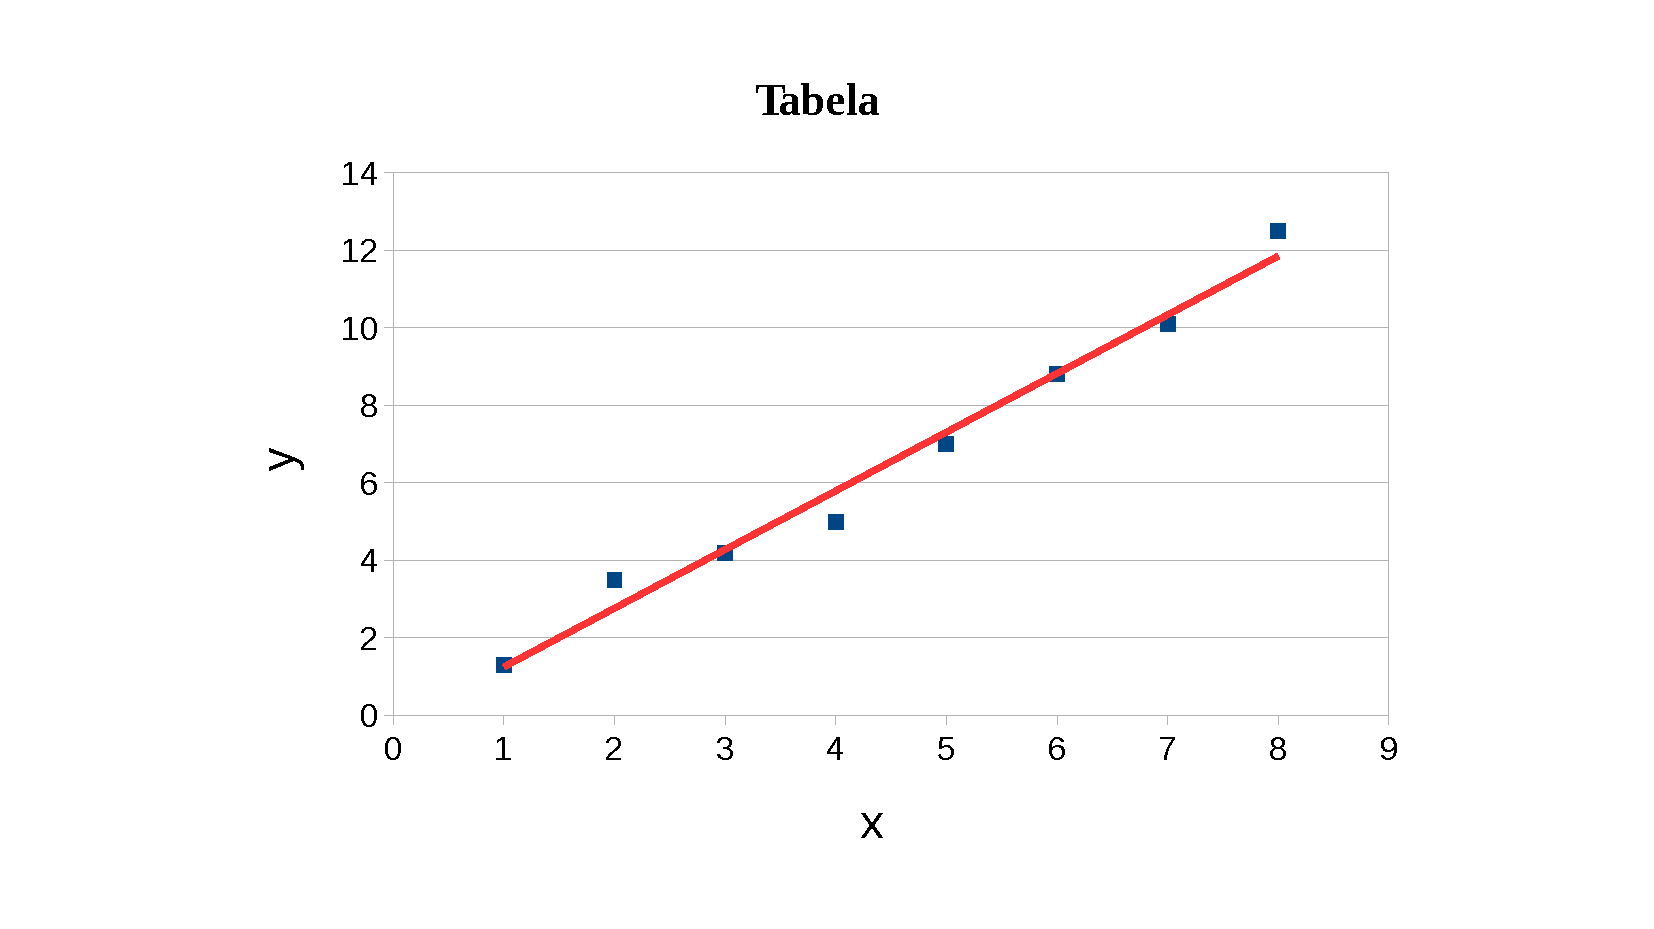
\includegraphics[height=\textheight-75pt]{images/tab-2}
            \end{center}
    \end{itemize}
\end{frame}

\begin{frame}
    \frametitle{Regressão Linear -- equações normais}
    Seja \(f(x) = ax + b\) a reta desejada. O métodos dos mínimos quadrados consiste em achar \(a\) e \(b\) que minimizem a função
    \[
        M(a,b) = \sum_{i=1}^n {\left(f(x_i) - yi\right)^2}
    \]

    \pause

    As equações normais para a regressão linear são

    \begin{align*}
        n b + a \sum_{i=1}^{n} {x_i} &= \sum_{i=1}^{n} {y_i} \\
        b \sum_{i=1}^{n} {x_i} + a \sum_{i=1}^{n} {x_i^2} &= \sum_{i=1}^{n} {x_iy_i}
    \end{align*}

    Elas formam um sistema linear que pode ser resolvido por eliminação de Gauss ou uma planilha eletrônica

\end{frame}

\begin{frame}
    \frametitle{Ajuste polinomial}

    Deseja-se encontrar um polinômio de grau \textit{n} que melhor se ajuste a \textit{m} pontos de uma tabela. Qual seria a forma das equações normais para esse caso?

    \pause
    \begin{block}
        {Função a ser minimizada}
        \[
            M (a_0,a_1, a_2, \ldots, a_n) = \sum_{i=1}^m {\left(
                    a_0 + a_1 x_i + a_2 x_i^2 + \cdots + a_n x_i^n
                    - yi
            \right)^2}
        \]
    \end{block}

    \pause
    \begin{block}
        {Equações normais}
        \[
            \sum_{k=0}^n a_k {\sum_{i=1}^m {x_i^{j+k}}} = \sum_{i=1}^m {y_i x_i^j}
        \]
        para \(j=0, 1, 2, \ldots, n\)
    \end{block}
\end{frame}

